\section{Motivation Behind the Research Work}

MPTCP is the most widely explored alternative for TCP, which supports multiple paths through multiple interfaces, while providing TCP like congestion control and reliability features for end-to-end connection. As mentioned earlier, a large number of researches~\cite{oh2016feedback,barik2016lisa,khalili2013mptcp,kheirkhah2016mmptcp,kheirkhah2015short} have explored MPTCP as an alternative of TCP for various application and network scenarios. However, MPTCP has two major shortcomings that prevent its large scale deployment over the Internet -- (a) MPTCP is implemented as a part of the Linux kernel, and therefore requires device reconfiguration for its deployment; and (b) MPTCP is still under exploration phase, and there are multiple shortcomings of MPTCP as pointed out by existing researches. In~\cite{khalili2013mptcp}, Khalili \textit{et al.} have claimed that MPTCP is not pareto optimal. Further, in~\cite{kheirkhah2016mmptcp}, the authors have pointed out that MPTCP is not suitable for short connections. 

Here, we first explore whether we can develop a MPTCP like protocol, or augment MPTCP so that we can support better network utilization for short flows. For this, we ask the following question: \textit{Why does MPTCP perform poorly for short flows?}  To get the answer, we do an emulation setup with the help of \texttt{Mininet} environment~\footnote{\url{http://mininet.org/} (last accessed: 24 April 2017)}, where we setup a network with two multi-homed hosts, and two distinct paths between the two hosts. We vary the end-to-end latency for the two paths, and then transfer data between the two hosts. For our experiment, we have configured the Linux kernel of the hosts with MPTCP version 0.91~\footnote{\url{http://multipath-tcp.org/} (last accessed: 24 April 2017)}. For this experiment, we set the path bandwidth as $50$ Mbps for both the paths. Among the two hosts, one host acts as the MPTCP server, while the other works as the MPTCP client. We keep a file at the server, and download that file from the client through MPTCP based connection. To observe the MPTCP behavior for various connection types, we vary the size of the file, and measure the impacts. 
%
%\begin{figure*}[ht]
%	\captionsetup[subfigure]{}
%	\begin{center}
%		\subfloat[\label{fig:percentSentOverPathRTT80}RTT=80ms]{
%			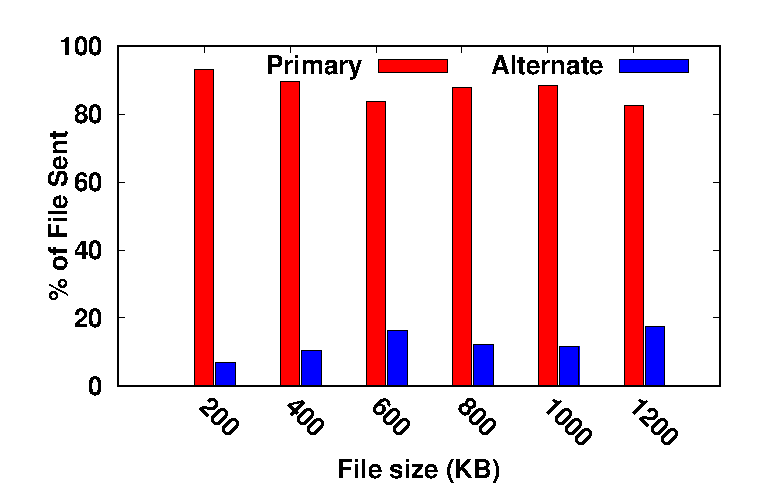
\includegraphics[width=0.32\linewidth]{img/exp4/delay-5}
%		}
%		\subfloat[\label{fig:percentSentOverPathRTT160}RTT=160ms]{
%			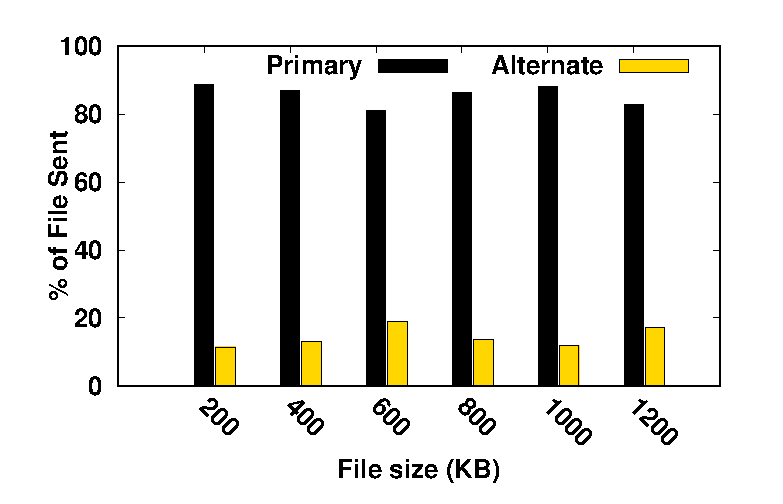
\includegraphics[width=0.32\linewidth]{img/exp4/delay-10}
%		}
%		\subfloat[\label{fig:percentSentOverPathRTT320}RTT=320ms]{
%			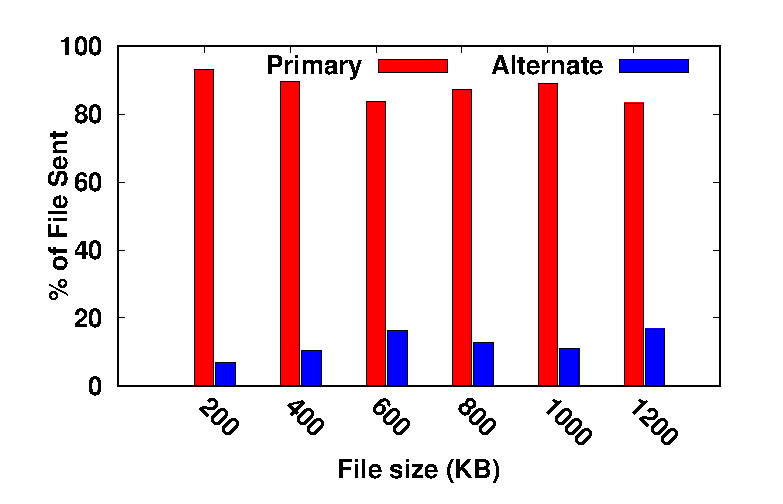
\includegraphics[width=0.32\linewidth]{img/exp4/delay-20}
%		}
%		
%		\caption{\label{fig:percentSentOverPath}\% of data share of a path.}
%	\end{center}
%\end{figure*}

\begin{figure}[!t]
	\begin{center}
	\begin{minipage}{0.45\linewidth}
		\centering
		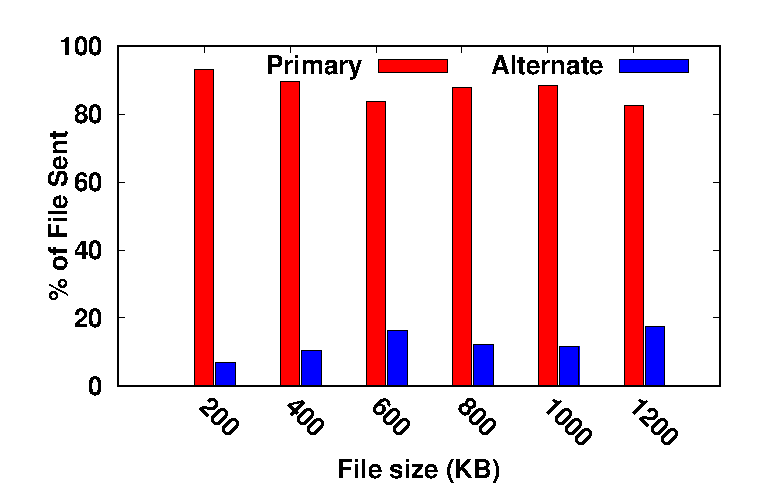
\includegraphics[width=\linewidth]{img/exp4/delay-5}
		\label{fig:percentSentOverPathRTT80}
		\subcaption{RTT=80ms}
	\end{minipage}
	\begin{minipage}{0.45\linewidth}
		\centering
		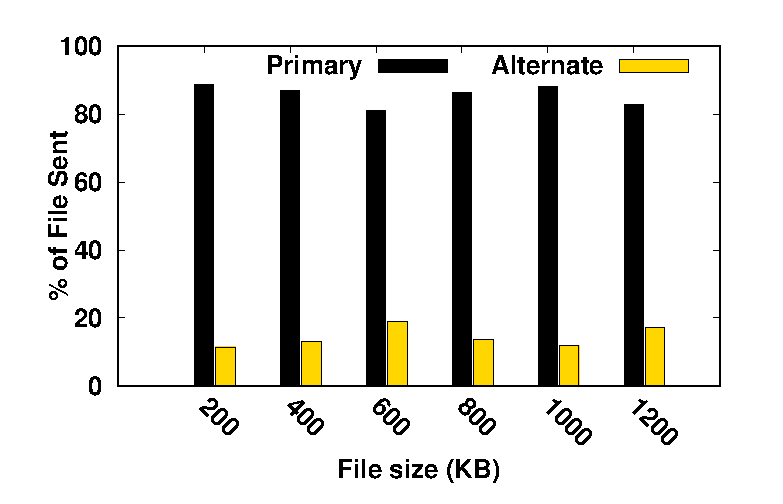
\includegraphics[width=\linewidth]{img/exp4/delay-10}
		\label{fig:percentSentOverPathRTT160}
		\subcaption{RTT=160ms}
	\end{minipage}
	\begin{minipage}{0.45\linewidth}
		\centering
		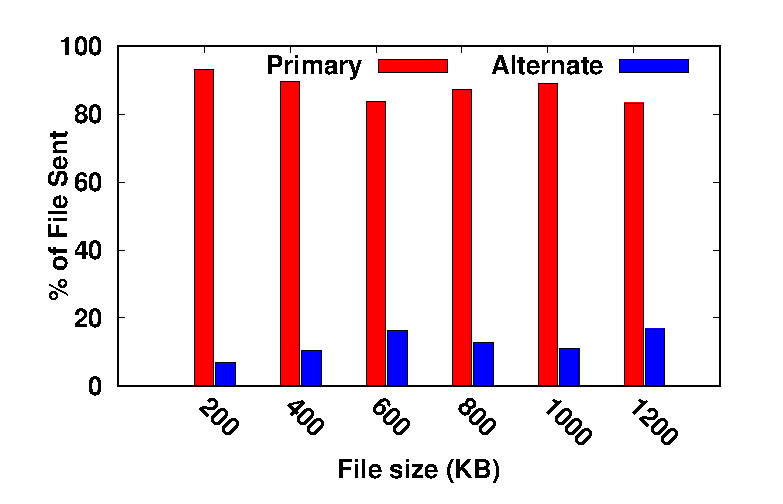
\includegraphics[width=\linewidth]{img/exp4/delay-20}
		\label{fig:percentSentOverPathRTT320}
		\subcaption{RTT=320ms}
	\end{minipage}
	\caption{\label{fig:percentSentOverPath}Percentage of Data Share between the Primary and the Alternate Paths}
	\end{center}
\end{figure}


\subsection{Utilization of Network Bandwidth at Alternate Paths for Short Flows}
MPTCP first initiates the connection through one of the available paths, called the {\em primary path}, and then explores the {\em alternate paths} to initiate alternate connections through them. In the first experiment, we try to look into the amount of data shares between the primary path and the alternate path. For this, we keep the bandwidth and latency for both the paths same, and vary the flow duration by increasing the size of the file to be downloaded at the client from the server. The results are plotted in Fig.~\ref{fig:percentSentOverPath}. We can observe from that figure that there is a huge imbalance between the two paths in terms of data share. The primary path forwards significantly more data compared to the alternate path. By exploring the connection logs, we find that by the time MPTCP sets up a connection to the alternate path, most of the data for a short flow has been transferred over the primary path. Further, the congestion controls for the primary and the alternate paths are handled separately, and therefore the alternate path also needs to go through the slow start phase. Therefore, the alternate path gets severely underutilized for short flows. Further, none of the primary sub-flow (sub-flow over the primary path) and the alternate sub-flow (sub-flow over the alternate path) can reach to the steady state for a short-lived flow.   

%
%We send the different sizes of data over from a host to another host via two separate paths in Mininet, where overall bandwidth and delay in the links are same for both the path. We find out that data share between two paths is imbalanced. We plot the results in Fig.~\ref{fig:percentSentOverPath}. We can see that 80\%-90\% of the data carries by primary path because \acrshort{mptcp} starts secondary sub-flow only after the establishment of the primary connection. By the time, secondary sub-flows establishes connection, primary sub-flow already sent several packets over the network. Primary sub-flow stays at least one \acrshort{rtt} ahead of secondary sub-flow. And none of the flow can reach the steady state for are short-lived flows.
%
%\acrshort{mptcp} can not balance between the different path for short-lived connection.

\subsection{Impact of MPTCP Path Selection During Connection Initiation}
We the perform another experiment on path selection, where the two paths have different round trip time (RTT). Here, we explore the effect of primary path selection, where we ask the following questions -- (a) {\em Does the RTT difference between the primary and the alternate path impact MPTCP performance?}; and (b) {\em Does the MPTCP performance differ if the low RTT path is selected as the primary path?} Consequently, we vary the RTT of the two paths, and the results are plotted in Fig.~\ref{fig:timeSentOverPath}. The two different bars in the graphs show the average file download time for two cases --  (i) low RTT path is used as the primary path, and (ii) high RTT path is used as the primary path. We observe that for small size file download, the performance varies a lot based on the selection of the primary path. However, the primary path selection is not a part of the core MPTCP mechanism, and MPTCP uses the path to set-up the primary sub-flow, which is provided by the underlying routing algorithm.  

%i.e. if \acrshort{mptcp} select longer path as primary path vs. shorter path as the primary path. In this experiment, we find that the time requires to send data using \acrshort{mptcp} over multiple paths largely depends on the primary path selection. For short-lived data and high RTT (Fig.~\ref{fig:timeSentOverPathRTT160}, Fig.~\ref{fig:timeSentOverPathRTT320}), it is taking significantly lesser time if \acrshort{mptcp} select shorter path as primary path. Results are plotted in Fig.~\ref{fig:timeSentOverPath}.
%\notesc{Do not use short and long paths -- use low RTT path and high RTT path in the figure. Use `File Size' instead of `Data Size'; and `Time Required to send Data' to `File Download Time'. }

%\begin{figure*}[ht]
%	\captionsetup[subfigure]{}
%	\begin{center}
%		\subfloat[\label{fig:timeSentOverPathRTT80}RTT: short path=80ms, long path=120ms]{
%			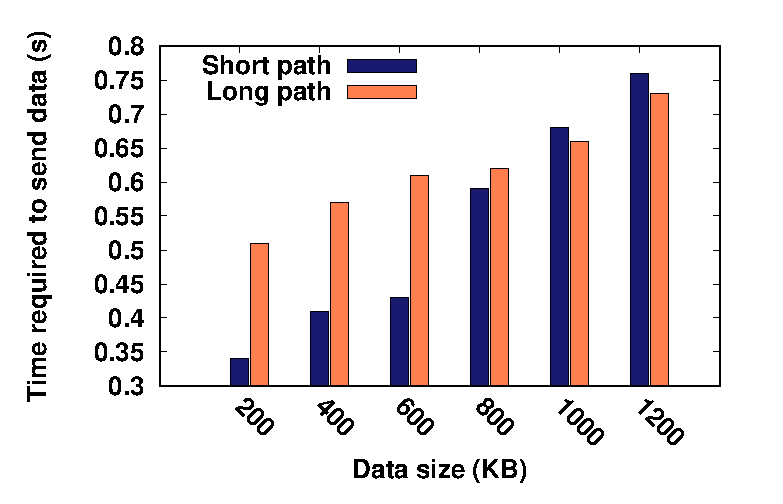
\includegraphics[scale=0.45]{img/exp5/time_needed_5}
%		}
%		\subfloat[\label{fig:timeSentOverPathRTT160}RTT: short path=160ms, long path=240ms]{
%			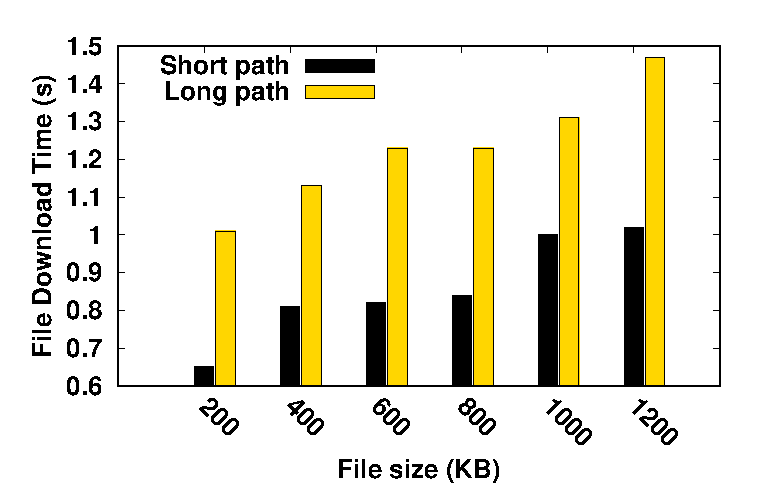
\includegraphics[scale=0.45]{img/exp5/time_needed_10}
%		}
%		\subfloat[\label{fig:timeSentOverPathRTT320}RTT: short path=320ms, long path=480ms]{
%			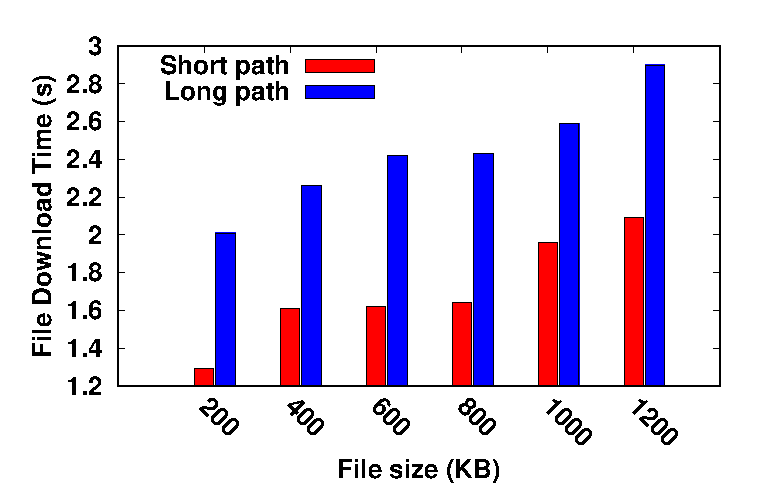
\includegraphics[scale=0.45]{img/exp5/time_needed_20}
%		}
%		
%		\caption{\label{fig:timeSentOverPath}Send data from client to server over 2 path using MPTCP. This is plot of \% of data went through a channel.}
%	\end{center}
%\end{figure*}

\begin{figure}[!t]
	\begin{center}
		\begin{minipage}{0.45\linewidth}
			\centering
			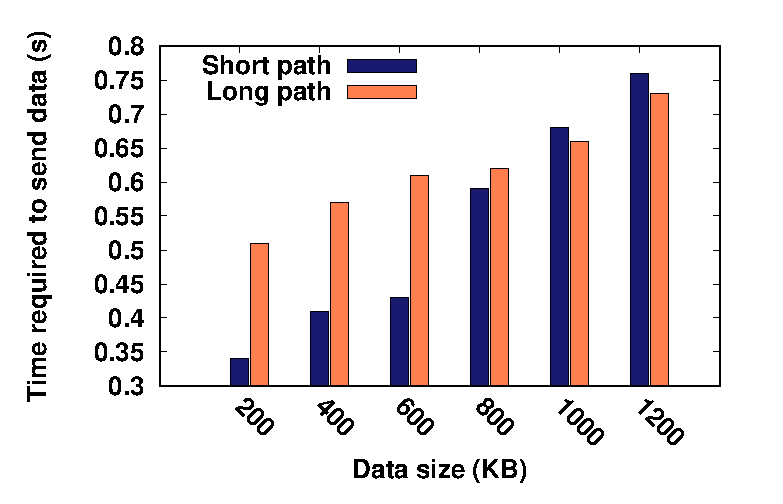
\includegraphics[width=\linewidth]{img/exp5/time_needed_5}
			\label{fig:timeSentOverPathRTT80}
			\subcaption{Short Path RTT: 80ms, Long Path RTT: 120ms}
		\end{minipage}
		\begin{minipage}{0.45\linewidth}
			\centering
			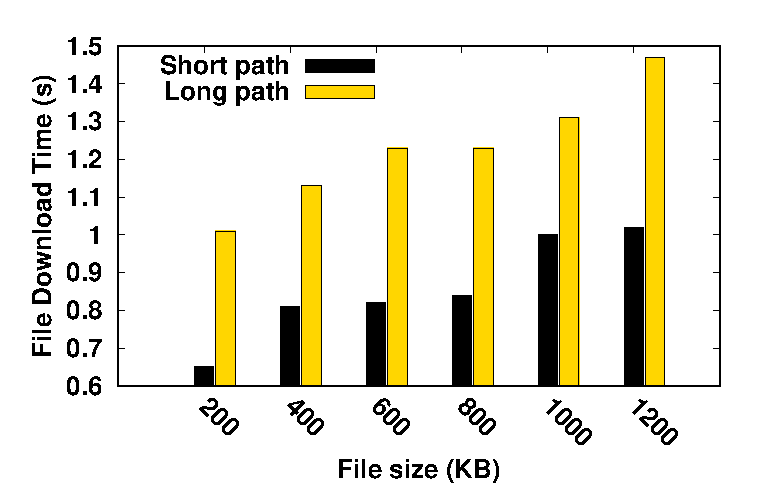
\includegraphics[width=\linewidth]{img/exp5/time_needed_10}
			\label{fig:timeSentOverPathPathRTT160}
			\subcaption{Short Path RTT: 160ms, Long Path RTT: 240ms}
		\end{minipage}
		\begin{minipage}{0.45\linewidth}
			\centering
			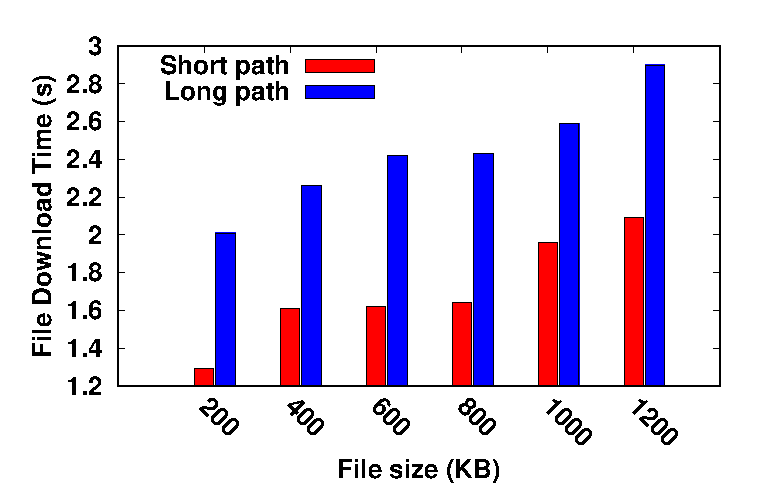
\includegraphics[width=\linewidth]{img/exp5/time_needed_20}
			\label{fig:timeSentOverPathRTT320}
			\subcaption{Short Path RTT: 320ms, Long Path RTT: 480ms}
		\end{minipage}
		\caption{\label{fig:timeSentOverPath}Difference in File Transmission Time based on the Primary Path Selection. The short path indicates the path with the low RTT value, whereas the long path indicates the path with the high RTT value}
	\end{center}
\end{figure}

%\acrshort{mptcp} is incapable of utilizing better path for short-lived connection if it makes mistakes in primary path selection. To overcome these issues and to use multipath, we developed \acrshort{udp} based multi-flow multipath protocol \textbf{Viscous}.
%
%In next section, we describe the protocol and how we overcome the problems with \acrshort{mptcp}.

\subsection{Take Aways}
In summary, the lessons learnt from the above experiments are as follows.
\begin{enumerate}
	\item Connection establishment time is an overhead for short flows. Further flow based congestion control algorithms results in the underutilization of network bandwidth, because every transport layer flow independently increases its transmission rate from the scratch (by increasing the congestion window value for TCP or MPTCP), and the flow may end before its transmission rate reaches to the network capacity. Flow multiplexing at the source device is important to handle such scenarios, however the HOL blocking problem needs to be avoided. 
	\item Connection establishment and path selection cannot be independent for a multi-path protocol, because the performance depends on the path selection mechanism. We need to develop a mechanism where the data transmission can be initiated simultaneously at multiple paths.   
\end{enumerate}
Accordingly, we target to develop a new transport wrapper as a part of this research, that works as a middleware between the application and the transport layer, and provides ubiquitous data transmission between two end hosts while ensuring reliability, flow control and congestion control.  The targeted protocol should use UDP as the transport protocol, and build up the services on top of that. 
%The detailed design philosophy of Viscous along with protocol specifications are discussed in the next section. 

%\newpage 